% Created 2019-08-27 mar 16:43
\documentclass[presentation,aspectratio=169]{beamer}
\usepackage[utf8]{inputenc}
\usepackage[T1]{fontenc}
\usepackage{fixltx2e}
\usepackage{graphicx}
\usepackage{longtable}
\usepackage{float}
\usepackage{wrapfig}
\usepackage{rotating}
\usepackage[normalem]{ulem}
\usepackage{amsmath}
\usepackage{textcomp}
\usepackage{marvosym}
\usepackage{wasysym}
\usepackage{amssymb}
\usepackage{hyperref}
\tolerance=1000
\usepackage{khpreamble}
\usepackage{amssymb}
\DeclareMathOperator{\shift}{q}
\DeclareMathOperator{\diff}{p}
\usetheme{default}
\author{Kjartan Halvorsen}
\date{2018-08-29}
\title{Computerized Control - discrete-time systems, z-transform}
\hypersetup{
  pdfkeywords={},
  pdfsubject={},
  pdfcreator={Emacs 25.3.50.2 (Org mode 8.2.10)}}
\begin{document}

\maketitle


\section{Intro}
\label{sec-1}


\begin{frame}[label=sec-1-1]{Result from quizz}
\begin{itemize}
\item Compute the z-transform
\item Pulse transfer function/operator
\item Modified z-transform
\end{itemize}
\end{frame}

\section{Discrete-time system example}
\label{sec-2}

\section{Zero-order hold, or step-invariant sampling}
\label{sec-3}
\begin{frame}[label=sec-3-1]{Impulse- step- and ramp-invariant sampling}
The idea is to sample the continuous-time system's response to a step input, in order to obtain a discrete approximation which is \alert{exact} (at the sampling instants) for such an input signal. 

\begin{center}
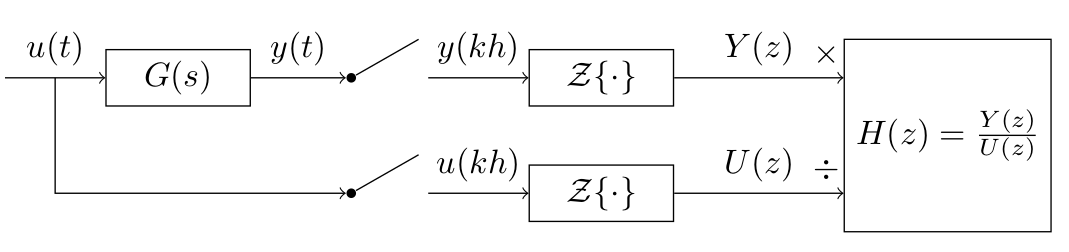
\includegraphics[width=0.7\linewidth]{../../figures/invariant-sampling.png}
\end{center}

\begin{itemize}
\item Impulse-invariant sampling: \( u(t) = \delta(t)\)
\item Step-invariant sampling (zero order hold): \( u(t) = \begin{cases} 1, & t \ge 0\\0, & t<0 \end{cases} \)
\item Ramp-invariant sampling: \( u(t) = \begin{cases} t, & t \ge 0\\0, & t<0 \end{cases} \)
\end{itemize}
\end{frame}


\begin{frame}[label=sec-3-2]{Step-invariant sampling, or zero-order-hold sampling}
Let the input to the continuous-time system be a step \(u(t)=\stepfcn,\) which has Laplace transform \(U(s)=\frac{1}{s}.\) In the Laplace-domain we get
\[Y(s) = G(s)\frac{1}{s}\]
\begin{enumerate}
\item Obtain the time-response by inverse Laplace: \(y(t)=\laplaceinv{Y(s)}\)
\item Sample the time-response to obtain the sequence \(y(kh)\) and apply  the z-transform to obtain \(Y(z) = \ztrf{y(kh)}\)
\item Calculate the pulse-transfer function by dividing with the z-transform of the input signal \(U(z) = \frac{z}{z-1}. \) \[H(z) = \frac{Y(z)}{U(z)} = \frac{z-1}{z}Y(z) \]
\end{enumerate}
\end{frame}

\begin{frame}[label=sec-3-3]{Example: First-order system}
Let's apply step-invariant sampling to the system
\[ G(s) = \frac{1}{s - \lambda}. \]
\end{frame}

\begin{frame}[label=sec-3-4]{Do on your own: The double integrator}
\[ G(s) = \frac{1}{s^2} \]
\end{frame}
% Emacs 25.3.50.2 (Org mode 8.2.10)
\end{document}